% !TEX root = ../main.tex

\section{Поняття випадкової величини}
Випадкова подія є якісною характеристикою можливого результату стохастичного експерименту.
Для успішного використання методів математичного аналізу в розв'язанні задач теорії ймовірностей
необхідно ввести кількісну характеристику випадкового результату стохастичного експерименту.
Такою характеристикою є \emph{випадкова величина} --- одне з основних понять теорії ймовірностей.
\begin{definition}\label{def:random_variable}
    Нехай $\left\{\Omega, \mathcal{F}, \P \right\}$ --- ймовірнісний простір деякого стохастичного експерименту.
    \emph{Випадковою величиною} називається функція $\xi = \xi(\omega): \Omega 
    \rightarrow \mathbb{R}$, для якої 
    \begin{equation}\label{eq:measurable}
        \forall x \in \mathbb{R}:
        \left\{ \omega \in \Omega\; :\; \xi(\omega) < x\right\} \in \mathcal{F}
    \end{equation} 
    В термінології функціонального аналізу умова \eqref{eq:measurable} означає, що функція $\xi(\omega)$ є
    \emph{вимірною відносно $\sigma$-алгебри $\mathcal{F}$}. Ця <<технічна>> вимога обґрунтована тим,
    що, як буде показано далі, саме ймовірності подій такого типу повністю характеризують випадкову величину.
\end{definition}
\begin{remark}
    Можна довести, що якщо виконується умова \eqref{eq:measurable}, то події виду
    $\left\{ \omega: \xi(\omega) > x\right\}$, $\left\{ \omega: \xi(\omega) \leq x\right\}$,
    $\left\{ \omega: \xi(\omega) \geq x\right\}$, $\left\{ \omega: \xi(\omega) = x\right\}$ та
    $\left\{ \omega: \xi(\omega) \in \left< a; b\right> \right\}$ також належать $\mathcal{F}$.
    Ідея доведення полягає у тому, що подія $\left\{ \omega: \xi(\omega) \geq x\right\}$ є
    доповненням до $\left\{ \omega: \xi(\omega) < x\right\}$ і тому належить $\mathcal{F}$
    за визначенням, подію $\left\{ \omega: \xi(\omega) > x\right\}$ (її доповнення --- 
    $\left\{ \omega: \xi(\omega) \leq x\right\}$) можна представити
    як зліченне об'єднання подій виду $\left\{ \omega: \xi(\omega) \geq x + \frac{1}{n}\right\}$
    та скористатися властивостями $\sigma$-алгебри.
    Нарешті, події виду $\left\{ \omega: \xi(\omega) = x\right\}$ та
    $\left\{ \omega: \xi(\omega) \in \left< a; b\right> \right\}$
    можна виразити як перетин вже розглянутих.
\end{remark}

Традиційно аргумент $\omega$ у позначенні випадкової величини не пишуть.
Випадкові величини будемо позначати малими літерами грецького алфавіту: $\xi$, $\eta$, $\zeta$ тощо.
Зауважимо, що для одного й того ж ймовірнісного простору можна задати безліч випадкових величин.
Наприклад, якщо стохастичний експеримент полягає в одноразовому підкиданні монети, елементарних подій лише дві
(якщо вважати, що на ребро монета ніколи не падає):
$\omega_1 = \left\{\text{випав герб}\right\}$ та $\omega_2 = \left\{\text{випала решка} \right\}$.
Можна задати незліченну множину випадкових величин за правилом $\xi_{x, y}(\omega_1) = x$ та
$\xi_{x, y}(\omega_2) = y$ для будь-яких $x, y\in\mathbb{R}$.

\begin{example}
    Наведемо ще приклади випадкових величин:
    \begin{enumerate}
        \item СЕ --- підкидання грального кубика один раз. Одними з можливих випадковими величин
        є кількість очок, що випала, парність (чи непарність) цієї кількості.
        \item СЕ --- проведення $N$ пострілів в мішень, однією з можливих випадкових величин є кількість влучень.
        \item СЕ --- вимірювання деякої невипадкової величини приладом. Випадковою величиною є значення похибки вимірювання.
        \item СЕ --- спостереження за роботою деякого приладу. Випадковою величиною є час безвідмовної роботи цього приладу.
    \end{enumerate}
\end{example}

%Надалі розглядатимуться випадкові величини двох видів --- дискретні (ДВВ) та неперервні (НВВ).

\subsection{Функція розподілу}

Універсальною ймовірнісною характеристикою будь-якої випадкової величини є функція 
розподілу випадкової величини.

\begin{definition}
    Дійснозначна функція дійсного аргументу $ F_\xi (x) = 
    \P\left\{\omega:\xi(\omega) < x\right\}$ або 
    $\P\left(\xi < x\right)$ називається \emph{функцією розподілу випадкової величини}.
\end{definition}

\noindent \textbf{Властивості функції розподілу:}
\begin{enumerate}
    \item Область визначення --- $\mathbb{R}$, область значень --- $\left<0; 1\right>$.
    \item $\forall x_1 > x_2 \in \mathbb{R}$: $ F_\xi(x_1) \geq F_\xi(x_2)$
    --- монотонно неспадна.
    \begin{proof}
        Розглянемо події $A = \left\{\omega:\xi(\omega) < x_1\right\}$ та 
        $B = \left\{\omega:\xi(\omega) < x_2\right\}$, причому $x_1 > x_2$.
        Отже, $B \subset A$, тому $\P(B) \leq \P(A)$ і $F_\xi(x_1) \geq F_\xi(x_2)$.
    \end{proof}
    \item $\P\left\{\omega: a \leq \xi(\omega) < b\right\} = F_\xi(b) - F_\xi(a)$.
    \begin{proof}
        Розглянемо події $A = \left\{\omega:\xi(\omega) < a\right\}$,  
        $B = \left\{\omega:\xi(\omega) < b\right\}$, 

        $C = \left\{\omega: a \leq \xi(\omega) < b\right\}$.
        $B = A \cup C, A \cap C = \varnothing$, тому $\P(B) = \P(A) + \P(C)$, звідки
        $\P(C) = \P\left\{\omega: a \leq \xi(\omega) < b\right\} 
        = \P(B) - \P(A) =  F_\xi(b) - F_\xi(a)$.
    \end{proof}
    \item \label{cdf:limit}$\lim\limits_{x \to -\infty} F_\xi(x) = 0, 
    \lim\limits_{x \to +\infty} F_\xi(x) = 1$.
    \begin{proof}
        Нехай $x_n$ --- деяка числова послідовність, що прямує до $+\infty$ (без втрати загальності --- додатна та монотонна).
        Введемо послідовності подій $A_n = \left\{\omega:\xi(\omega) 
        < -x_n\right\}$ та
        $B_n = \left\{\omega:\xi(\omega) < x_n\right\}$. Зауважимо, що $A_n$ є 
        монотонно спадною, а $B_n$ --- монотонно зростаючою,
        причому $\bigcap\limits_{n=1}^\infty A_n = \varnothing$,
        $\bigcup\limits_{n=1}^\infty B_n = \Omega$, бо $\xi$ приймає лише скінченні значення.

        $\lim\limits_{n \to \infty} F_\xi(-x_n) = \lim\limits_{n \to \infty} 
        \P(A_n)
        = \left[\;\parbox{7.5em}{ теорема\\ неперервності \refeq{th:2}}\right] = 
        \P\left(\bigcap\limits_{n=1}^\infty A_n\right) = \P(\varnothing) = 0$.

        $\lim\limits_{n \to +\infty} F_\xi(x_n) = \lim\limits_{n \to +\infty} 
        \P(B_n)
        = \left[\;\parbox{7.5em}{ теорема\\ неперервності \refeq{th:1}}\right] = 
        \P\left(\bigcup\limits_{n=1}^\infty B_n\right) = \P(\Omega) = 1$.

        Оскільки $x_n$ була довільною, то $\lim\limits_{x \to -\infty} F_\xi(x) = 0$ і
        $\lim\limits_{x \to +\infty} F_\xi(x) = 1$.
    \end{proof}
    \item \label{cdf:left_con} Функція розподілу неперервна зліва: $\lim\limits_{x \to x_0 - 0} 
    F_\xi(x) = F_\xi(x_0)$.
    \begin{proof}
        Нехай $x_n$ --- деяка числова послідовність, що прямує до $x_0$ зліва,
        тобто $x_n < x_0$ для всіх $n$ (і є монотонною без втрати загальності). Введемо послідовність подій
        $A_n = \left\{\omega: \xi(\omega) < x_n\right\}$, яка є зростаючою. Тоді
        
        $\lim\limits_{n\to\infty} 
        F_\xi(x_n) = \lim\limits_{n \to \infty}\P(\xi < x_n) =
        \left[\;\parbox{7.5em}{ теорема\\ неперервності \refeq{th:2}}\right]
         = \P\left(\bigcup\limits_{n=1}^\infty A_n\right)  = \P(\xi < x_0) = F_\xi(x_0)$.
        Знову з довільності $x_n$ отримуємо $\lim\limits_{x \to x_0-0} F_\xi(x) = F_\xi(x_0)$.
    \end{proof}
    \item Розглянемо ймовірність $\P\left\{x \leq \xi < x + \Delta x\right\} = F_\xi (x+\Delta x) - F_\xi (x)$.
    Перейдемо до границі при $\Delta x \rightarrow 0$:
    $\P\left\{ \xi = x\right\} = \begin{cases}
        0, & \text{якщо } x \text{ --- точка неперервності} \\
        \Delta \text{-стрибок}, & \text{якщо } x \text{ --- точка розриву 1-го роду}
    \end{cases}$.
\end{enumerate}

\begin{remark}
    В іноземній літературі функція розподілу іноді вводиться інакше,
    як $F_\xi (x) = \P\left\{\omega:\xi(\omega) \leq x\right\}$.
    За такого означення вона є неперервною справа.
\end{remark}

\subsection{Дискретні випадкові величини}
\begin{definition}
    Випадкова величина $\xi$ називається 
    \emph{дискретною випадковою величиною (ДВВ)}, якщо вона набуває скінченну або зліченну 
    кількість значень. Функція розподілу ДВВ, відповідно, має скінченну або зліченну кількість розривів першого роду.
\end{definition}
Для задання ДВВ, крім знання значень випадкової величини, необхідно знати ймовірності, 
з якими ці значення приймаються.
$$p_i = \P\left\{\omega: \xi(\omega) = x_i\right\} = \P(\xi = x_i) > 0, i = 1,2,... , \; \sum\limits_{i=1}^\infty p_i = 1$$

\begin{definition}
    \emph{Законом розподілу (ймовірностей)} ДВВ називається співвідношення, яке вказує, 
    які значення ця випадкова величина приймає та з якими ймовірностями.
    Закон розподілу ДВВ записується у вигляді \emph{ряду розподілу}:
    \vspace{0.5em}
    
    \hspace{30pt}
    \begin{tabular}{|c|c|c|c|c|c|}
        \hline
        $\xi$ & $x_1$ & $x_2$ & ... & $x_n$ & ... \\
        \hline
        $p$ & $p_1$ & $p_2$ & ... & $p_n$ & ... \\
        \hline
    \end{tabular}
    \hspace{40pt}
    $x_1 < x_2 < ... < x_n < ...,\; \sum\limits_i p_i = 1$
\end{definition}
\begin{example}
    $\xi$ задає кількість влучень при чотирьох пострілах з імовірністю влучення 
    $p = \frac{1}{2}$. Скласти закон розподілу цієї випадкової величини.

    З формули Бернуллі \eqref{eq:bern_prob} $\P(\xi = k) = C_4^k \left(\frac{1}{2}\right)^k \left(\frac{1}{2}\right)^{4-k} = 
    C_4^k \left(\frac{1}{2}\right)^4 = \frac{C_4^k}{2^4}, k = 0,1,2,3,4$, тому маємо такий ряд розподілу:

    \begin{center}
        \begin{tabular}{|c|c|c|c|c|c|}
            \hline
            $\xi$ & 0 & 1 & 2 & 3 & 4 \\
            \hline
            $p$ & $1/2^4$ & $4/2^4$ & $6/2^4$ & $4/2^4$ & $1/2^4$ \\
            \hline
        \end{tabular}
    \end{center}
\end{example}
\begin{definition}
    Графічне зображення закону розподілу ДВВ називається 
    \emph{полігоном розподілу ймовірностей}.
\end{definition}

\hbox to \hsize{\hfil{
    \begin{tikzpicture}
        \pgfmathsetmacro{\s}{0.6};
        \pgfmathsetmacro{\t}{1.5};
        \draw [->] (0,0) -- (6*\t,0);
        \draw [->] (0,0) -- (0,6*\s);
        \draw [fill] (1*\t, 0) circle [radius = 0.05];
        \node [below] at (1*\t, 0) {$x_1$};
        \node [below] at (2*\t, 0) {$x_2$};
        \node [below] at (3*\t, 0) {$x_3$};
        \node [below] at (3.75*\t, 0) {$...$};
        \node [below] at (4.5*\t, 0) {$x_n$};
        \node [below] at (5.25*\t, 0) {$...$};
        \node [left] at (0, 1*\s) {$p_1$};
        \node [left] at (0, 2*\s) {$p_3$};
        \node [left] at (0, 3*\s) {$p_2$};
        \node [left] at (0, 3.75*\s) {$...$};
        \node [left] at (0, 4.5*\s) {$p_n$};
        \draw [fill] (2*\t, 0) circle [radius = 0.05];
        \draw [fill] (3*\t, 0) circle [radius = 0.05];
        \draw [fill] (4.5*\t, 0) circle [radius = 0.05];
        \draw [fill] (0, 1*\s) circle [radius = 0.05];
        \draw [fill] (0, 2*\s) circle [radius = 0.05];
        \draw [fill] (0, 3*\s) circle [radius = 0.05];
        \draw [fill] (0, 4.5*\s) circle [radius = 0.05];
        \draw [fill] (0, 5.5*\s) circle [radius = 0.05];
        \node [left] at (0, 5.5*\s) {$1$};
        \node [right] at (6*\t, 0) {$x$};
        \node [above] at (0, 6*\s) {$p$};
        \draw [dashed] (0, 5.5*\s) -- (6*\t, 5.5*\s);
        \draw [fill] (1*\t, 1*\s) circle [radius = 0.05];
        \draw [fill] (2*\t, 3*\s) circle [radius = 0.05];
        \draw [fill] (3*\t, 2*\s) circle [radius = 0.05];
        \draw [fill] (4.5*\t, 4.5*\s) circle [radius = 0.05];
        \draw [thick] (1*\t, 1*\s) -- (2*\t, 3*\s) -- (3*\t, 2*\s);
        \draw [thick] (3*\t, 2*\s) -- (3.5*\t, 2.8333*\s);
        \draw [thick, dashed] (3.5*\t, 2.8333*\s) -- (4*\t, 3.6667*\s);
        \draw [thick] (4*\t, 3.6667*\s) -- (4.5*\t, 4.5*\s) -- (5.25*\t, 4*\s);
        \draw [thick, dashed] (5.25*\t, 4*\s) -- (5.75*\t, 3.6667*\s);
    \end{tikzpicture}
}\hfil}

\noindent \textbf{Вигляд функції розподілу для ДВВ.}
Як вже було зазначено, функція розподілу ДВВ має скінченну або зліченну кількість розривів першого роду
в точках, які відповідають значенням, які величина може набувати.
\nopagebreak
\begin{center}
    \begin{tabular}{c c}
        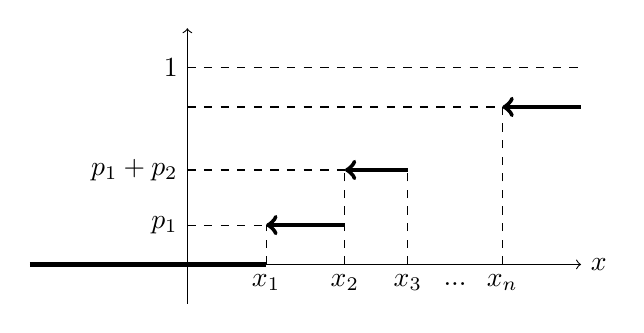
\begin{tikzpicture}[baseline={(current bounding box.center)}]
            \draw [->] (-2, 0) -- (5, 0);
            \draw [->] (0, -0.5) -- (0, 3);
            \draw [ultra thick] (-2, 0) -- (1, 0);
            \draw [dashed] (1, 0) -- (1, 0.5);
            \draw [ultra thick] [<-] (1, 0.5) -- (2, 0.5);
            \draw [dashed] (2, 0) -- (2, 1.2);
            \draw [ultra thick] [<-] (2, 1.2) -- (2.8, 1.2);
            \draw [dashed] (2.8, 0) -- (2.8, 1.2);
            \draw [dashed] (4, 0) -- (4, 2);
            \draw [ultra thick] [<-] (4, 2) -- (5, 2);
            \draw [dashed] (0, 2.5) -- (5, 2.5);
            \draw [dashed] (0, 0.5) -- (1, 0.5);
            \draw [dashed] (0, 1.2) -- (2, 1.2);
            \draw [dashed] (0, 2) -- (4, 2);
            \node [below] at (1, 0) {$x_1$};
            \node [below] at (2, 0) {$x_2$};
            \node [below] at (2.8, 0) {$x_3$};
            \node [below] at (3.4, -0.1) {$...$};
            \node [below] at (4, 0) {$x_n$};
            \node [left] at (0, 0.5) {$p_1$};
            \node [left] at (0, 1.2) {$p_1 + p_2$};
            \node [left] at (0, 2.5) {$1$};
            \node [right] at (5, 0) {$x$};
        \end{tikzpicture} &
        $F_\xi(x) = \begin{cases}
            0, & x \leq x_1 \\
            p_1, & x_1 < x \leq x_2 \\
            p_1 + p_2, & x_2 < x \leq x_3 \\
            \dots \\
            \sum\limits_{i=1}^{n} p_i, & x_{n} < x \leq x_{n+1} \\
            \dots
        \end{cases}$
    \end{tabular}
\end{center}
Якщо ДВВ набуває лише скінченну кількість значень, то $F_\xi(x) = 1$ при $x>x_n$.

\subsection{Неперервні випадкові величини}
\begin{definition}
    Випадкова величина $\xi$ називається \emph{неперервною випадковою величиною (НВВ)},
    якщо її функція розподілу неперервна, диференційовна майже скрізь, можливо, за виключенням
    окремих ізольованих точок.
\end{definition}
\begin{remark}
    Існують і інші класи випадкових величин, крім ДВВ та НВВ. Якщо функція розподілу
    монотонно зростає на деяких проміжках і має розриви першого роду в окремих точках,
    то така випадкова величина називається \emph{мішаною}. Також можна побудувати величину,
    яка не буде ані дискретною, ані неперервною, ані мішаною --- так звану \emph{сингулярну} випадкову величину.
    Надалі будемо розглядати лише ДВВ та НВВ.
\end{remark}
З неперервності функції розподілу для довільної точки $x_0$ маємо $\P\left\{\xi = x_0\right\} = 0$.
Замість ймовірності потрапляння НВВ у окрему точку розглядається так звана щільність розподілу ймовірностей у цій точці.

\begin{definition}
    \emph{Щільність розподілу ймовірностей} неперервної випадкової величини $\xi$
    дорівнює границі (якщо вона існує):
    \begin{equation}\label{eq:prob_dens}
        \lim_{\Delta x\rightarrow 0} \frac{\P\left\{x\leq \xi < x+\Delta x\right\}}{\Delta x}
    \end{equation}
\end{definition}
Отже, закон розподілу НВВ можна задавати щільністю $f_\xi(x) = \lim\limits_{\Delta x\rightarrow 0} \frac{\P\left\{x\leq \xi < x+\Delta x\right\}}{\Delta x}$.
Нескладно помітити \emph{зв'язок щільності з функцією розподілу}:
\begin{equation}\label{eq:dens_pdf}
    f_\xi(x) = \lim\limits_{\Delta x\rightarrow 0} \frac{\P\left\{x\leq \xi < x+\Delta x\right\}}{\Delta x} = 
    \lim\limits_{\Delta x\rightarrow 0} \frac{F_\xi(x+\Delta x) - F_\xi(x)}{\Delta x} = F'_\xi(x)
\end{equation}
\begin{definition}
    Графік щільності розподілу називається \emph{кривою розподілу}.
\end{definition}

\vspace{0.5em}
\noindent \textbf{Властивості щільності розподілу:}
\begin{enumerate}
    \item Область визначення $D(f) = \mathbb{R}$, область значень $E(f) = \left[0; +\infty\right)$, оскільки $F_\xi(x)$ є монотонно неспадною.
    \item $F_\xi(x)=\int\limits_{-\infty}^x f_\xi(t)dt$.
    \begin{proof}
        З формули Ньютона-Лейбніца $\int\limits_{-\infty}^x f_\xi(t)dt = F_\xi(x) - \underset{x\to-\infty}{\lim}F_\xi(x) = F_\xi(x)$.
    \end{proof}
    \item \emph{Властивість нормування:} оскільки $\lim\limits_{x \to +\infty} F_\xi(x) = 1$, то $\int\limits_{-\infty}^{+\infty} f_\xi(x)dx = 1$.
    Геометрична інтерпретація цієї властивості --- площа під кривою розподілу завжди рівна $1$.
    \item $\P\left\{\omega: a \leq \xi(\omega) < b\right\} = F_\xi(b) - F_\xi(a) = \int\limits_a^b f_\xi(x)dx$.
    Ця властивість справджується і для довільних проміжків $\left< a; b\right>$,
    оскільки, як вже було сказано, ймовірності потрапляння в окремі точки рівні 0. Геометрично це означає,
    що ймовірність потрапляння в будь-який проміжок $\left< a; b\right>$ дорівнює площі криволінійної трапеції,
    обмеженої кривою розподілу, віссю абсцис та прямими $x=a$, $x=b$.
\end{enumerate}

\begin{example}
    \begin{enumerate}
        \item Нехай $f_\xi(x) = \begin{cases}
            0, & x \notin \left[1; 3\right] \\
            A\cdot x^2, & x \in \left[1; 3\right]
        \end{cases}$. Знайти $A$ та $F_\xi(x)$.

        \begin{tabular}{c p{7cm}}
            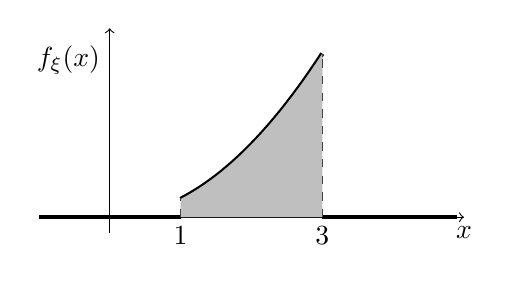
\begin{tikzpicture}[baseline={(current bounding box.north)}, yscale = 2, xscale=0.9]
                \draw [->] (-1, 0) -- (5, 0);
                \draw [->] (0, -0.1) -- (0, 1.2);
                \draw [ultra thick] (-1, 0) -- (1, 0);
                \draw [dashed] (1, 0) -- (1, 0.115384615385);
                \draw [dashed] (3, 0) -- (3, 1.03846153846);
                \draw [ultra thick] (3, 0) -- (4.9, 0);
                \draw [domain=1:3, smooth, variable = \x, ultra thick] plot ({\x}, {0.115384615385 * \x * \x});
                \node [below] at (1, 0) {$1$};
                \node [below] at (3, 0) {$3$};
                \node [below] at (5, 0) {$x$};
                \node [left] at (0, 1) {$f_\xi(x)$};
                \fill [lightgray, domain=1:3, variable = \x] (1, 0) -- plot ({\x}, {0.115384615385 * \x^2}) -- (3, 0) -- cycle;
            \end{tikzpicture} &
                $\int\limits_{-\infty}^{+\infty} f_\xi(x)dx = A\cdot\int\limits_1^3 x^2 dx = 
                A\cdot \frac{x^3}{3} \bigr\vert_1^3 = A\cdot \frac{26}{3}$.
            
                З властивості нормування $A = \frac{3}{26}$.
        \end{tabular}

        \begin{tabular}{c c}
            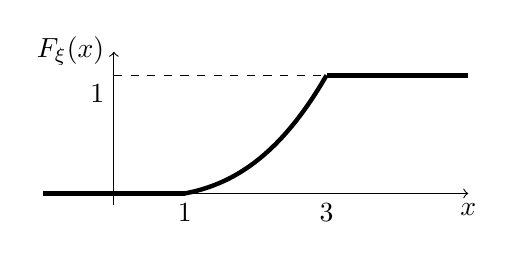
\begin{tikzpicture}[baseline={(current bounding box.center)}, yscale = 1.5, xscale=0.9]
                \draw [->] (-1, 0) -- (5, 0);
                \draw [->] (0, -0.1) -- (0, 1.2);
                \draw [ultra thick] (-1, 0) -- (1, 0);
                \draw [domain=1:3, smooth, variable = \x, ultra thick] plot ({\x}, {0.0384615384615 * (\x^3-1)});
                \draw [ultra thick] (3, 1) -- (5, 1);
                \draw [dashed] (0, 1) -- (5, 1);
                \node [below] at (1, 0) {$1$};
                \node [below] at (3, 0) {$3$};
                \node [below left] at (0, 1) {$1$};
                \node [below] at (5, 0) {$x$};
                \node [above left] at (0, 1) {$F_\xi(x)$};
            \end{tikzpicture} &
            $ F_\xi(x) = \int\limits_{-\infty}^x f_\xi(t)dt = \begin{cases}
                0, \; x \leq 1 \\
                \int\limits_{-\infty}^1 0dt + \int\limits_1^x \frac{3}{26}t^2dt = \\
                \frac{1}{26}(x^3-1), \; 1 < x \leq 3 \\
                \int\limits_{-\infty}^1 0dt + \int\limits_1^3 \frac{3}{26}t^2dt + \\
                + \int_3^x 0 dt = 1, \;x > 3
            \end{cases}$
        \end{tabular}
        \item Щільність розподілу може мати розриви 2-го роду:
        \nopagebreak
        \begin{center}
            \begin{tabular}{c c}
                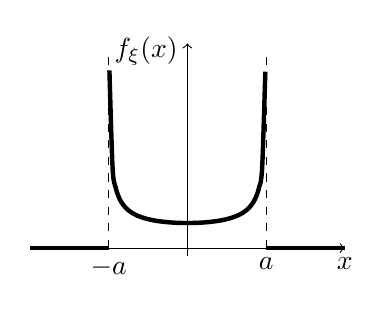
\begin{tikzpicture}[baseline={(current bounding box.center)}]
                    \draw [->] (-2, 0) -- (2, 0);
                    \draw [->] (0, -0.1) -- (0, 2.6);
                    \draw [ultra thick] (-2, 0) -- (-1, 0);
                    \draw [ultra thick] (1, 0) -- (2, 0);
                    \draw [dashed] (-1, 0) -- (-1, 2.5);
                    \draw [dashed] (1, 0) -- (1, 2.5);
                    \draw [samples=50, domain=-0.99:0.99, smooth, variable = \x, ultra thick] plot ({\x}, {1/(3.14159265359 * sqrt(1 - \x * \x)});
                    \node [below] at (2, 0) {$x$};
                    \node [left] at (0, 2.5) {$f_\xi(x)$};
                    \node [below] at (-1, 0) {$-a$};
                    \node [below] at (1, 0) {$a$};
                \end{tikzpicture} &
                $f_\xi(x) = \begin{cases}
                    0, & \vert x \vert \geq a \\
                    \frac{1}{\pi\sqrt{a^2-x^2}}, & \vert x \vert < a
                \end{cases}$          
            \end{tabular}
        \end{center}

        Відповідна функція розподілу (так званий <<закон арксинуса>>) дорівнює
        \begin{gather*}
            F_\xi(x) = \begin{cases}
                0, & x\leq -a \\
                \frac{1}{\pi}\int\limits_{-a}^x \frac{1}{\sqrt{a^2-t^2}} dt = 
                \frac{1}{\pi}\left(\arcsin\left(\frac{x}{a}\right) + \frac{\pi}{2}\right), & -a < x \leq a \\
                1, & x > a
            \end{cases}
        \end{gather*}
    \end{enumerate}
\end{example}